\documentclass{article}
\usepackage[utf8]{inputenc}
\usepackage[T1]{fontenc}
\usepackage{graphicx}
\usepackage{hyperref}
\usepackage{geometry}
\geometry{margin=1in}

\title{SWORN BORSHAS ((after juradi}
\date{Encyclopaedia Britannica (1771)}

\begin{document}
\maketitle

\section*{Historical source}
\textbf{Entry ID:} \texttt{entry-sworn-borshas-after-juradi-251} \\
\textbf{Volume ID:} 191679021 \\
\textbf{Character Count:} 464

\subsection*{Extracted Text}
SWORN BORSHAS ((after juradi), perfonió, by
manual oath, overward to flare each others fortune. For-
metly, in any notable question in invade and concuer en
summits country, it was the culton for the more eminent ful
diers to engage themselves by reciprocal oaths to fame the
revards of their device. This practice gave cocotion to the
growth of \_Jones brothers to freedom in majority,\_ because of
their dividing plunder and fpalt.

SYCOMORFrans, has发言. See Acces.



\section*{Source record}
\begin{itemize}
\item \textbf{Dataset:} \texttt{NationalLibraryOfScotland/encyclopaedia\_britannica\_illustrated}
\item \textbf{Dataset Revision:} \texttt{309f765b1ecc83e0a7f7762e44b4a927a7555443}
\item \textbf{Page ID:} \texttt{britannica:309f765b1ecc83e0a7f7762e44b4a927a7555443:train:251} \\
  \textbf{Filename:} \texttt{page-0251-69952e7c4a0f.jpg} \\
  \textbf{Row Index:} 251 \\
  \textbf{SHA256:} \texttt{69952e7c4a0f4026...}
\end{itemize}

\begin{figure}[h]
\centering
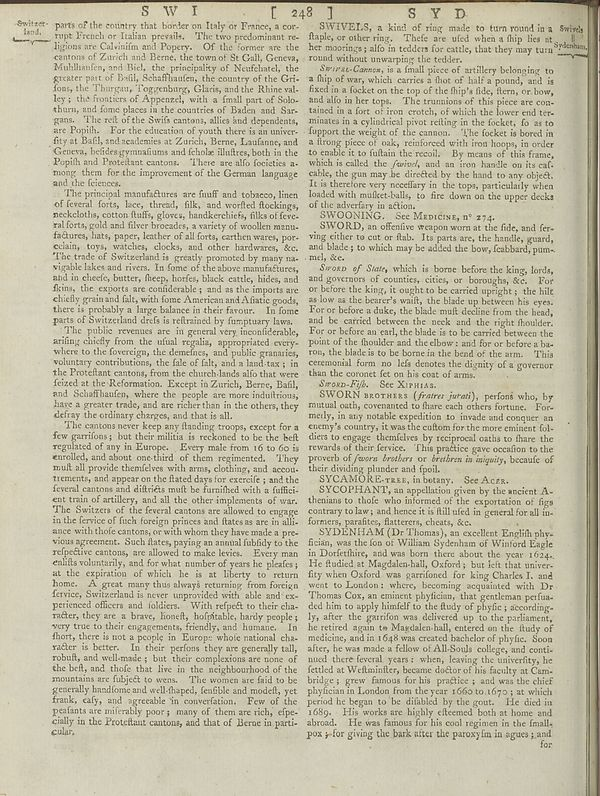
\includegraphics[width=0.85\textwidth]{../scans/page-0251-69952e7c4a0f.jpg}
\caption*{Source scan: \texttt{page-0251-69952e7c4a0f.jpg}}
\end{figure}

\end{document}
